\documentclass[a4paper, titlepage]{article}

\usepackage[ngerman]{babel}
\usepackage[T1]{fontenc}
\usepackage[utf8]{inputenc}
\usepackage{graphicx}
\usepackage{amsmath}
\usepackage{tabularx}
\usepackage{siunitx}

\newcommand{\accunit}[1]{\SI{#1}{\metre\per\square\second}}


\title{Die Gravitationskonstante g
auf einer schiefen Bahn bestimmen}
\author{Sascha Huber, Aaron Stampa, Joanne Gautschi, Damien Flury}
\date{1. Dezember 2019}
\begin{document}
    \maketitle
    \tableofcontents
    \newpage
    \section{Einleitung}
    Die Gravitation begleitet den Mensch tagtäglich. Doch wie stark
    ist sie auf der Erde eigentlich und wie kann sie bestimmt werden?
    Diese Frage hat sich bereits Galileo Galilei anfang des 17. Jahrhunderts
    gestellt. Da er jedoch keine Möglichkeit hatte, die
    Zeit sehr genau zu bestimmen, konnte er dies nicht auf der
    Vertikale tun (die Beschleunigung ist zu hoch). Somit nahm er
    sich eine schiefe Bahn zur Hilfe und konnte dann mit einfacher
    Mathematik eine ungefähre Näherung an die Gravitationskonstante $g$
    berechnen. Sie bezeichnet die Beschleunigung, die ein Körper nahe
    der Erde im freien Fall erreicht (ohne Einberechnung des 
    Luftwiderstandes) und beträgt nach heutigen Forschungen
    etwa \accunit{9.81}.

    Wir möchten ähnliche Versuche ausführen und somit $g$ ungefähr bestimmen. 
    Um eine praktische Sicht auf $g$ zu zeigen, werden wir als Anfangsexperiment einen
    vertikalen Fall analysieren. Dazu verwenden wir zunächst unseren eigenen
    Herzschlag und eine mechanische Uhr (ungefähr die Messmethode, 
    welche Galileo hatte), um die Zeit zu bestimmen, welche ein Ball
    benötigt, um zwei Meter in die Tiefe zu fallen. Da uns mittlerweile
    wesentlich genauere Messmethoden zur Verfügung stehen, bestimmen wir
    die Zeit im Anschluss mit einer Stoppuhr, welche eine Genauigkeit bis im 
    Millisekundenbereich aufweist.
    
    In einem weiteren Experiment verwenden wir einen Bewegungssensor, um
    die Beschleunigung von Objekten auf einer schiefen Bahn zu bestimmen
    und Excel, um diese in einer Tabellenform darzustellen. Wie in 
    Abbildung \ref{incline} dargestellt, können wir durch Messen des
    Weges $x$ und der Höhe $h$ anhand von Trigonometrie den Neigungswinkel
    $\theta$ bestimmen. Mehr dazu später im Artikel.






    \begin{figure}
        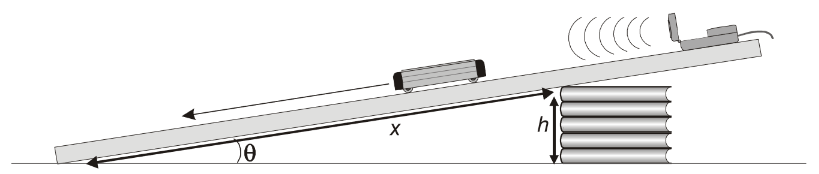
\includegraphics[width=\textwidth]{images/incline.png}
        \caption{Schiefe Bahn}
        \label{incline}
    \end{figure}








    \section{Experiment}
    Wir haben unser Experiment eingerichtet, wie auf Abbildung
    \ref{incline} dargestellt. Dann haben wir verschiedene Objekte
    herunterrollen lassen mit verschieden Höhen
    \emph{h}. Die Länge \emph{x} ist die Distanz, in welcher
    wir die Objekte messen. Der Winkel $\theta$ bezeichnet
    den Winkel der schiefen Ebene in Bogenmass.

    \subsection{Ball auf der schiefen Ebene}
    Zunächst haben wir einen Ball herunterrollen lassen.
    Sein Radius \emph{r} beträgt etwa 4 cm, seine Masse
    \emph{m} 242 g.
    
    Wir haben die Strecke \emph{s} in Abhängigkeit
    der Zeit \emph{t} gemessen, um die Beschleunigung
    \emph{a} zu bestimmen. Dazu haben wir folgende Formel
    angewandt:
    \begin{align}
        s &= \frac{1}{2} \cdot a \cdot t^2 \\
        a &= \frac{2 \cdot s}{t^2} &\text{(Termumformung)}
    \end{align}



    \begin{table}
        \begin{tabularx}{\textwidth}{|X|X|X|X|X|X|X|}
            \hline
            \textbf{Number of books} & \textbf{Height of books $(m)$} & 
            \boldmath{$\sin{\theta}$} & \textbf{Trial 1}
            (\accunit{}) & 
            \textbf{Trial 2} (\accunit{}) & 
            \textbf{Trial 3} (\accunit{}) & 
            \textbf{Average acceleration} (\accunit{}) \\
            \hline
            3 & 0.115 & 0.0479 & 0.26 & 0.31 & 0.36 & 0.310 \\
            \hline
            4 & 0.144 & 0.0600 & 0.49 & 0.38 & 0.41 & 0.426 \\
            \hline
            5 & 0.174 & 0.726 & 0.60 & 0.45 & 0.38 & 0.476 \\
            \hline
            6 & 0.200 & 0.834 & 0.61 & 0.59 & 0.56 & 0.586 \\
            \hline
            7 & 0.275 & 0.115 & 0.97 & 1.22 & 1.22 & 1.137 \\
            \hline
        \end{tabularx}
        \caption{Messwerte (Ball)}
    \end{table}


\end{document}